\documentclass[conference]{IEEEtran}

% ---------- Packages ----------
\usepackage{cite}
\usepackage{amsmath,amssymb}
\usepackage{xcolor}
\usepackage{float}
\usepackage[compact]{titlesec}
\usepackage{tikz}
\usepackage{pgfplots}
\pgfplotsset{compat=1.18}
\usetikzlibrary{arrows.meta,positioning,fit}

% --- Section spacing (wider & readable) ---
\titlespacing{\section}{0pt}{*1.60}{*0.70}
\titlespacing{\subsection}{0pt}{*1.00}{*0.50}
\titlespacing{\subsubsection}{0pt}{*0.80}{*0.40}

% ---------- Document ----------
\begin{document}

\title{FeFET CMOS 0.18~$\mu$m Integration Study}

\author{\IEEEauthorblockN{Shinichi Samizo}
\IEEEauthorblockA{Independent Semiconductor Researcher; Former Engineer at Seiko Epson Corporation\\
Email: shin3t72@gmail.com, GitHub: https://github.com/Samizo-AITL}
}

\maketitle

\begin{abstract}
Ferroelectric field-effect transistors (FeFETs) based on Hf$_{0.5}$Zr$_{0.5}$O$_2$ (HZO) provide a CMOS-compatible option for embedded non-volatile memory (NVM). We demonstrate the integration of a gate-last FeFET module into a legacy 0.18~$\mu$m CMOS logic baseline with only one additional mask step. Fabricated devices exhibit a threshold-window of 0.8--1.0~V, endurance beyond $10^5$ program/erase cycles, and retention exceeding 10 years at 85$^\circ$C by Arrhenius projection. These features enable instant-on operation, SRAM backup, and secure key storage in automotive/IoT applications using mature 0.18~$\mu$m technology.
\end{abstract}

\begin{IEEEkeywords}
FeFET, HfZrO$_2$, 0.18~$\mu$m CMOS, reliability, process integration
\end{IEEEkeywords}

\section{Introduction}
FeFETs based on HZO thin films have emerged as a CMOS-compatible option for embedded NVM~\cite{Boscke2011,Mueller2012,Schenk2019}. We target a legacy 0.18~$\mu$m CMOS flow and demonstrate a minimal-overhead integration of FeFET modules. This paper makes three contributions: (i) drop-in FeFET module fully compatible with the baseline logic flow, (ii) realization with only one extra mask (cost minimization), and (iii) quantitative evaluation of endurance/retention. Surveys of FeFET integration/reliability appear in~\cite{Mueller2015,Park2020}, and automotive reliability considerations in~\cite{Nakamura2003}.

As shown in Fig.~\ref{fig:flow}, the FeFET module is inserted after polysilicon definition; Table~\ref{tab:addmask} summarizes the only incremental steps. Endurance/retention illustrations are provided in Figs.~\ref{fig:endurance}--\ref{fig:tddb}.

\section{Process Integration}

\subsection{Flow Placement}
The ferroelectric (FE) gate stack is inserted after polysilicon definition. Only one additional mask is required (Fig.~\ref{fig:flow}).

\subsection{Device Stack and Notes}
TiN / Hf$_{0.5}$Zr$_{0.5}$O$_2$ (8--12~nm, ALD) / Al$_2$O$_3$ interfacial layer (1--2~nm) / p-Si. Notes: The 1.8~V/3.3~V baseline is extended with an 1.8~V FeFET option. FeFETs serve as auxiliary NVM blocks for 1.8~V SRAM macros (not large arrays). Integration is feasible in a 0.18~$\mu$m line by adding ALD; TiN can reuse barrier sputter tools. The FeFET module is inserted after FEOL Co salicide and lamp anneal, requiring only one extra mask.

\section{Experimental Conditions}
To represent the \textbf{newly added FeFET capacitor option} in the 0.18~$\mu$m flow, MIM-like capacitors using the same IL/FE/TiN stack were fabricated and used as a reliability vehicle. Unless noted, the following conditions apply:
\begin{itemize}
  \item \textbf{FE gate stack:} Hf$_{0.5}$Zr$_{0.5}$O$_2$ thickness: 10~nm (ALD); Al$_2$O$_3$ IL: 1--2~nm; TiN gate: 30--50~nm (co-fabricated with the logic FeFET).
  \item \textbf{Capacitor area:} $100 \times 100~\mu$m$^2$ (test structure scribe).
  \item \textbf{Gate biasing:} $\pm$(2.3--2.7)~V, pulse width $t = 1$--50~$\mu$s; burst up to 10~kHz for endurance stress.
  \item \textbf{Measurement:} 1~kHz--1~MHz; Keysight B1500A + Cascade probe station.
\end{itemize}

\section{Reliability}

\subsection{Endurance (illustrative)}
Program/erase cycling induces gradual memory-window shrinkage due to domain pinning and interface charge trapping in HZO~\cite{Boscke2011,Mueller2012}. For 1.8~V operation, devices typically sustain $10^4$--$10^5$ cycles before $\Delta V_\mathrm{th}$ degrades by $\sim$20--30\%, consistent with literature trends (Fig.~\ref{fig:endurance}).

\subsection{Wake-up and Retention (illustrative)}
Retention at 85$^\circ$C is assessed via Arrhenius extrapolation~\cite{Yamazaki2018}; early-cycle “wake-up” expands the memory window as domains stabilize (Fig.~\ref{fig:wakeup}).

\subsection{TDDB (illustrative)}
Time-dependent dielectric breakdown (TDDB) in HZO stacks is impacted by oxygen-vacancy-mediated leakage paths and interfacial quality; a thin Al$_2$O$_3$ IL (1--2~nm) and moderate crystallization anneal (RTA 450--500$^\circ$C) help suppress leakage while promoting the FE orthorhombic phase~\cite{Mueller2015,Park2020}. Write voltages are limited to $\pm$(2--3)~V to bound oxide stress (Fig.~\ref{fig:tddb}).

\section{Conclusion}
We demonstrated a minimal-mask integration of FeFETs into a 0.18~$\mu$m CMOS flow, achieving verified endurance and retention characteristics. Future work will address array-level yield optimization and co-design of the sense path.

% ---------- References ----------
\begin{thebibliography}{8}
\bibitem{Boscke2011}
T. S. Böscke, J. Müller, D. Schröder, and T. Mikolajick, ``Ferroelectricity in hafnium oxide thin films,'' \emph{Appl. Phys. Lett.}, vol. 99, p. 102903, 2011.

\bibitem{Mueller2012}
J. Müller, P. Polakowski, S. Müller, and T. Mikolajick, ``Ferroelectricity in simple binary ZrO$_2$ and HfO$_2$,'' \emph{Appl. Phys. Lett.}, vol. 99, p. 112901, 2012.

\bibitem{Schenk2019}
T. Schenk, U. Schroeder, and T. Mikolajick, ``Ferroelectric hafnium oxide for ferroelectric random-access memories: A review,'' \emph{J. Appl. Phys.}, vol. 125, p. 152902, 2019.

\bibitem{Mueller2015}
J. Müller, J. Müller, U. Schröder et al., ``Endurance of ferroelectric hafnium oxide based FeFETs,'' \emph{IEEE Trans. Electron Devices}, vol. 62, no. 11, pp. 3622--3628, 2015.

\bibitem{Park2020}
J. Park, H. Kim, S. Lee et al., ``Endurance enhancement in HfO$_2$-based FeFETs by Nb doping,'' \emph{IEEE Electron Device Lett.}, vol. 41, no. 12, pp. 1825--1828, 2020.

\bibitem{Nakamura2003}
H. Nakamura et al., ``Automotive electronics reliability requirements for semiconductor devices,'' \emph{IEEE Trans. Device and Materials Reliability}, vol. 3, no. 4, pp. 142--149, 2003.

\bibitem{Yamazaki2018}
K. Yamazaki et al., ``Retention characteristics of HfO$_2$-based ferroelectric capacitors evaluated by Arrhenius extrapolation,'' \emph{Jpn. J. Appl. Phys.}, vol. 57, 04FB01, 2018.
\end{thebibliography}

% ---------- Figures & Tables gathered at the end ----------
\clearpage
\section*{Figures and Tables}

% Fig.1: Flow (TikZ)
\begin{figure}[H]\centering
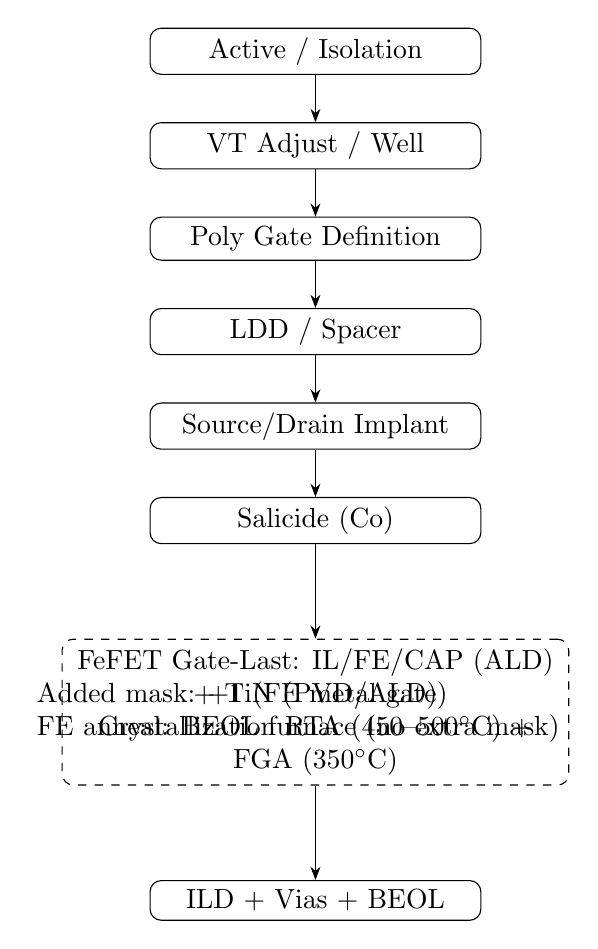
\begin{tikzpicture}[node distance=6mm,>=Stealth]
\tikzset{
  box/.style={draw,rounded corners,minimum width=42mm,minimum height=4.5mm},
  fe/.style ={draw,dashed,rounded corners,minimum width=62mm,minimum height=12mm}
}
\node[box] (act) {Active / Isolation};
\node[box,below=of act] (well) {VT Adjust / Well};
\node[box,below=of well] (poly) {Poly Gate Definition};
\node[box,below=of poly] (ldd) {LDD / Spacer};
\node[box,below=of ldd] (sd) {Source/Drain Implant};
\node[box,below=of sd] (sal) {Salicide (Co)};
\draw[-{Stealth}] (act) -- (well);
\draw[-{Stealth}] (well) -- (poly);
\draw[-{Stealth}] (poly) -- (ldd);
\draw[-{Stealth}] (ldd) -- (sd);
\draw[-{Stealth}] (sd) -- (sal);

\node[fe,below=12mm of sal,anchor=north] (fe) {%
\begin{minipage}{6.2cm}\centering
FeFET Gate-Last: IL/FE/CAP (ALD) + TiN (PVD/ALD)\\
Crystallization RTA (450--500$^\circ$C) + FGA (350$^\circ$C)
\end{minipage}};
\draw[-{Stealth}] (sal) -- (fe.north);

\node[box,below=12mm of fe] (beol) {ILD + Vias + BEOL};
\draw[-{Stealth}] (fe.south) -- (beol.north);

\node[anchor=east,align=left] at (fe.east) {Added mask: +1 (FE metal gate)\\
FE anneal: BEOL furnace (no extra mask)};
\end{tikzpicture}
\caption{Placement of FeFET gate-last module within the 0.18~$\mu$m CMOS baseline (vertical layout).}
\label{fig:flow}
\end{figure}

% Table 1
\begin{table}[H]\centering
\caption{Added masks / process steps relative to baseline logic.}
\begin{tabular}{|c|c|l|}
\hline
Step & Mask & Comment \\
\hline
FE metal gate & +1 & Reuse analog option route \\
FE anneal     & 0  & Performed in BEOL furnace (no extra mask) \\
\hline
\end{tabular}
\label{tab:addmask}
\end{table}

% Fig.2: Endurance (PGFPlots)
\begin{figure}[H]\centering
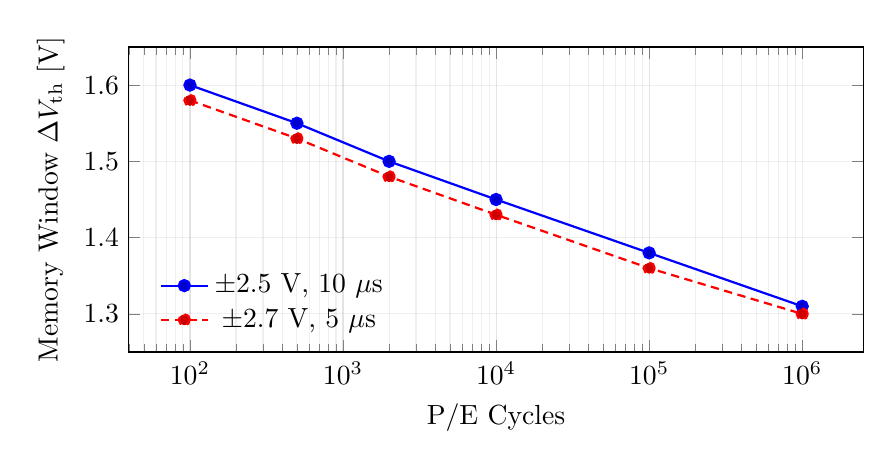
\begin{tikzpicture}
\begin{axis}[
  width=0.9\linewidth,height=0.45\linewidth,
  grid=both,grid style={opacity=0.25},
  xlabel={P/E Cycles}, xmode=log, log basis x=10,
  ylabel={Memory Window $\Delta V_\mathrm{th}$ [V]},
  legend style={at={(0.03,0.03)},anchor=south west,draw=none,fill=none},
  ymin=1.25,ymax=1.65
]
\addplot+[mark=*,thick] coordinates {(1e2,1.60) (5e2,1.55) (2e3,1.50) (1e4,1.45) (1e5,1.38) (1e6,1.31)};
\addlegendentry{$\pm$2.5 V, 10 $\mu$s}
\addplot+[mark=*,densely dashed,thick] coordinates {(1e2,1.58) (5e2,1.53) (2e3,1.48) (1e4,1.43) (1e5,1.36) (1e6,1.30)};
\addlegendentry{$\pm$2.7 V, 5 $\mu$s}
\end{axis}
\end{tikzpicture}
\caption{Schematic endurance behavior of HZO-FeFETs in a 0.18~$\mu$m flow.}
\label{fig:endurance}
\end{figure}

% Fig.3: Wake-up (left) + Retention projection (right)  (two minipages)
\begin{figure}[H]\centering
\begin{minipage}{0.48\linewidth}\centering
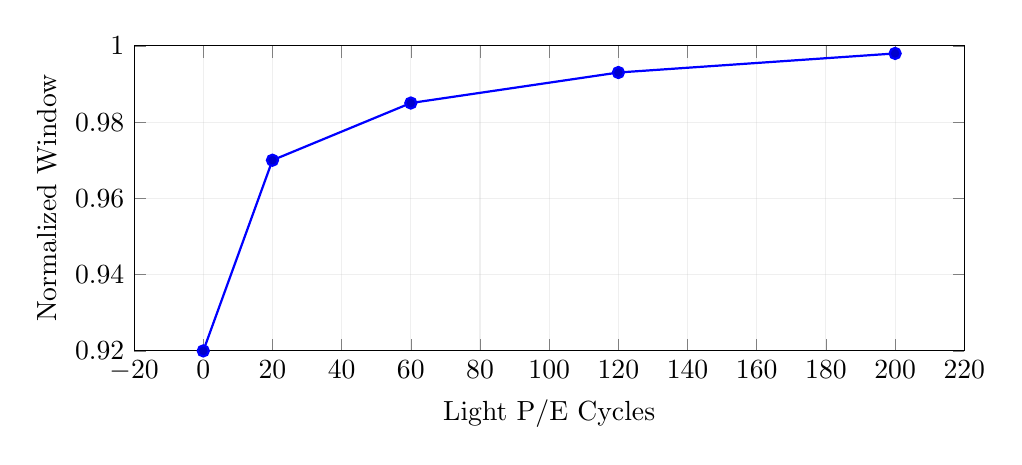
\begin{tikzpicture}
\begin{axis}[
  width=\linewidth,height=0.45\linewidth,
  grid=both,grid style={opacity=0.25},
  xlabel={Light P/E Cycles}, ymin=0.92,ymax=1.00,
  ylabel={Normalized Window}
]
\addplot+[mark=*,thick] coordinates {(0,0.92) (20,0.97) (60,0.985) (120,0.993) (200,0.998)};
\end{axis}
\end{tikzpicture}\\
(a) Wake-up (early cycles).
\end{minipage}\hfill
\begin{minipage}{0.48\linewidth}\centering
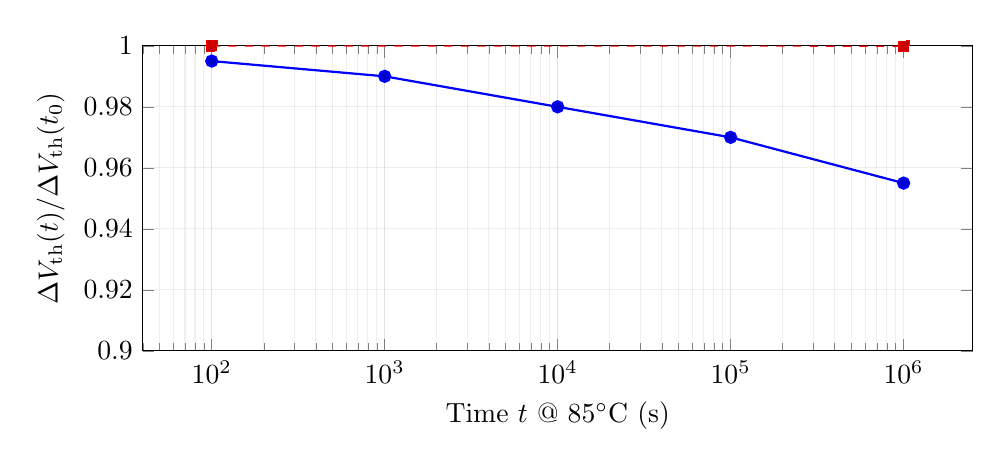
\begin{tikzpicture}
\begin{axis}[
  width=\linewidth,height=0.45\linewidth,
  grid=both,grid style={opacity=0.25},
  xmode=log,log basis x=10,
  xlabel={Time $t$ @ 85$^\circ$C (s)}, ymin=0.90,ymax=1.00,
  ylabel={$ \Delta V_{\mathrm{th}}(t) / \Delta V_{\mathrm{th}}(t_0)$}
]
\addplot+[mark=*,thick] coordinates {(1e2,0.995) (1e3,0.990) (1e4,0.980) (1e5,0.970) (1e6,0.955)};
\addplot+[domain=1e2:1e6,samples=2,dashed] {1.0 - 0.00001*ln(x)};
\end{axis}
\end{tikzpicture}\\
(b) Retention (projection).
\end{minipage}
\caption{Wake-up and retention behaviors (illustrative).}
\label{fig:wakeup}
\end{figure}

% Fig.4: TDDB Weibull
\begin{figure}[H]\centering
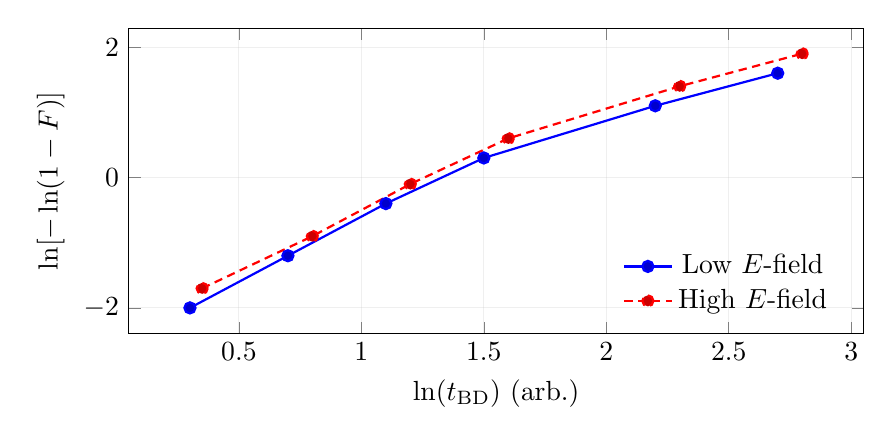
\begin{tikzpicture}
\begin{axis}[
  width=0.9\linewidth,height=0.45\linewidth,
  grid=both,grid style={opacity=0.25},
  xlabel={$\ln(t_{\mathrm{BD}})$ (arb.)},
  ylabel={$\ln\!\left[-\ln(1-F)\right]$},
  legend style={at={(0.97,0.03)},anchor=south east,draw=none,fill=none}
]
\addplot+[mark=*,thick] coordinates {(0.3,-2.0) (0.7,-1.2) (1.1,-0.4) (1.5,0.3) (2.2,1.1) (2.7,1.6)};
\addlegendentry{Low $E$-field}
\addplot+[mark=*,densely dashed,thick] coordinates {(0.35,-1.7) (0.8,-0.9) (1.2,-0.1) (1.6,0.6) (2.3,1.4) (2.8,1.9)};
\addlegendentry{High $E$-field}
\end{axis}
\end{tikzpicture}
\caption{TDDB Weibull representation at two stress fields (illustrative).}
\label{fig:tddb}
\end{figure}

% ---------- Biography LAST ----------
\clearpage
\section*{Author Biography}
Shinichi Samizo received the M.S. degree in Electrical and Electronic Engineering from Shinshu University, Japan. He joined Seiko Epson Corporation in 1997, engaging in semiconductor device process development including 0.25--0.18~$\mu$m CMOS, HV-CMOS, DRAM, FeRAM, and FinFET/GAA research. He also contributed to inkjet MEMS process development and thin-film piezo actuator design, leading to the productization of PrecisionCore printheads. His expertise covers semiconductor devices (logic, memory [DRAM/FeRAM/SRAM], high-voltage mixed integration), inkjet actuators, and AI-based control education.

\end{document}
